\documentclass{beamer}
\usetheme{Madrid} % Выбор темы
\usecolortheme{seahorse} % Выбор цветовой схемы

\usepackage{amsmath} % американское математическое сообщество.
\usepackage{amssymb} % миллион разных значков и готический, ажурный шрифты.
\usepackage{amscd} % диаграммы, графики.
\usepackage{amsthm} % окружения теорем, определений и тд.
\usepackage{physics} % основные физические символы
%\usepackage{latexsym} % треугольники и пьяная стрелка.

%пакеты для шрифтов:
%\usepackage{euscript} % прописной шрифт с завитушками.
\usepackage{MnSymbol} % Значеки дaxs[i//n, i%n]ельства
\usepackage{verbatim} % улучшенный шрифт "пишущей машинки".
%\usepackage{array} % более удобные таблицы.
%\usepackage{multirow} % мультистолбцы в таблицах.
%\usepackage{longtable} % таблицы на несколько страниц.
%\usepackage{latexsym}
\usepackage{tikz-feynhand} % Феймановские диограммы


\usepackage{hyphenat}
\usepackage{etoolbox}
\usepackage{collectbox} % Добавляет коробочки, можно складывать туда текст)



%Пакеты для оформления:
\RequirePackage[center, medium]{titlesec}% Стиль секций и заголовков
%\usepackage[x11names]{xcolor} % 317 новых цветов для текста.
%\usepackage{multicol} % набор текста в несколько колонн.
%\usepackage{breqn} % мультистоки в урвнениях 
\usepackage{anyfontsize}
\usepackage{graphicx} % расширенные возможности вставки стандартных картинок.
\usepackage{subcaption} % возможность вставлять картинки в строчку
%\usepackage{caption} % возможность подавить нумерацию у caption.
\usepackage{wrapfig} % вставка картинок и таблиц, обтекаемых текстом.
\usepackage{cancel} % значки для сокращения дробей, упрощения, стремления.
\usepackage{multirow}
%\usepackage{misccorr} % в заголовках появляется точка, но при ссылке на них ее нет.
%\usepackage{indentfirst} % отступ у первой строки раздела
%\usepackage{showkeys} % показывает label формул над их номером.
%\usepackage{fancyhdr} % удобное создание верхних и нижних колонтитулов.
%\usepackage{titlesec} % еще одно создание верхних и нижних колонтитулов

%Пакеты шрифтов, кодировок. НЕ МЕНЯТЬ РАСПОЛОЖЕНИЕ.
\usepackage[utf8x]{inputenc} % кодировка символов.
%\usepackage{mathtext} % позволяет использовать русские буквы в формулах. НЕСОВМЕСТИМО С tempora.
\usepackage[T1, T2A]{fontenc} % кодировка шрифта.
\usepackage[english, russian]{babel} % доступные языки.


%Сокращения
\newcommand{\piv}[2]{\cfrac{\partial #1}{\partial #2}}


%Скобочки
\newcommand{\inrad}[1]{\left( #1 \right)}
\newcommand{\inner}[1]{\left( #1 \right)}
\newcommand{\infig}[1]{\left\{ #1 \right\}}
\newcommand{\insqr}[1]{\left[ #1 \right]}
\newcommand{\ave}[1]{\left\langle #1 \right\rangle}


%% Красивые <= и >=
\renewcommand{\geq}{\geqslant}
\renewcommand{\leq}{\leqslant}

%%Значек выполнятся
\newcommand{\per}{\hookrightarrow}


%% Более привычные греческие буквы
\renewcommand{\phi}{\varphi}
\renewcommand{\epsilon}{\varepsilon}
\newcommand{\eps}{\varepsilon}
\newcommand{\Eps}{\mathfrak{E}}
\newcommand{\com}{\mathbb{C}}
\newcommand{\re}{\mathbb{R}}
\newcommand{\nat}{\mathbb{N}}
\newcommand{\stp}{$\filledmedtriangleleft$}
\newcommand{\enp}{$\filledmedsquare$}


\newcommand{\mergelines}[2]{
\begin{tabular}{llp{.5\textwidth}}
    #1 \\ #2
\end{tabular}
}
\newcommand\tab[1][0.51cm]{\hspace*{#1}}
\newcommand\difh[2]{\frac{\partial #1}{\partial #2}}

    

\title{Измерение формактора распада $\Lambda_c \to \Lambda l \nu_l $}
\author[Карибджанов Матвей]{\underline{Карибджанов Матвей}, Пахлов Павел}
    
\begin{document}

\begin{frame}% первый слайд
    \titlepage
\end{frame}

\begin{frame}{Мотивация}
    \begin{itemize}
        \item Уточнение результата CLEO. Improved measurement of the form-factors in the decay
        $\Lambda^+_c \to \Lambda e \nu_e$ J. W. Hinson et al. // Phys. Rev. Lett. — 2005. — Vol. 94. — Iss. 19, 191801. — 5 p.
        \item  Проверка моделей HQET, LQCD проедсказывающие формфакторы распада $\Lambda_c \to \Lambda$.
    \end{itemize}
\end{frame}

\begin{frame}{Теория}
    \begin{figure}[H]
        \centering
        \begin{tikzpicture}
            \begin{feynhand}
                \vertex [particle] (i1) at (-3,4) {$u$};
                \vertex [particle] (i2) at (-3,3.5) {$d$};
                \vertex [particle] (i3) at (-3,3) {$c$};
                \vertex [particle] (f1) at (3,4) {$u$};
                \vertex [particle] (f2) at (3,3.5) {$d$};
                \vertex [particle] (f3) at (3,3) {$s$};
                \vertex (w1) at (0,3);
                \vertex (w2) at (0,2.5);
                \vertex (w3) at (0,2);
                \vertex (w4) at (1.5,1);
                \vertex [particle] (e) at (3,1.5) {$l^{-}$};
                \vertex [particle] (an) at (3,0.5) {$\bar{\nu}_{l}$};
                \propag [fermion] (i1) to (w1);
                \propag [fermion] (i2) to (w2);
                \propag [fermion] (i3) to (w3);
                \propag [fermion] (w1) to (f1);
                \propag [fermion] (w2) to (f2);
                \propag [fermion] (w3) to (f3);
                \propag [charged boson] (w3) to [edge label=$W^{-}$] (w4);
                \propag [fermion] (w4) to (e);
                \propag [anti fermion] (w4) to (an);        
            \end{feynhand}
        \end{tikzpicture}
    \end{figure}
    \begin{eqnarray*}
        \bra{B_{\Lambda_c}}
        j_\nu^V
        \ket{B_{\Lambda}} = 
        u_\Lambda^\dag \inner{\mathfrak F^V_1 \inner{q^2} \gamma_\nu + 
        \cfrac{\mathfrak F^V_2}{M_{\Lambda_c}} \inner{q^2} \sigma_{\mu\nu} q^\nu + 
        \cfrac{\mathfrak F^V_3}{M_{\Lambda_c}} \inner{q^2} q_\mu} u_{\Lambda_c} \\
        \bra{B_{\Lambda_c}}
        j_\nu^A
        \ket{B_{\Lambda}} = 
        u_\Lambda^\dag \inner{\mathfrak F^A_1 \inner{q^2} \gamma_\nu + 
        \cfrac{\mathfrak F^A_2}{M_{\Lambda_c}} \inner{q^2} \sigma_{\mu\nu} q^\nu + 
        \cfrac{\mathfrak F^A_3}{M_{\Lambda_c}} \inner{q^2} q_\mu} \gamma_5 u_{\Lambda_c} 
        \label{eq:def_form}
    \end{eqnarray*}
\end{frame}

\begin{frame}{Теория}
    \begin{equation*}
        H_{\lambda_\Lambda \lambda_w} = H^V_{\lambda_\Lambda \lambda_w} 
        + H^A_{\lambda_\Lambda \lambda_w} 
    \end{equation*}
     
    \begin{equation*}
        H^{V,A}_{\lambda_\Lambda \lambda_w} = 
        \bra{B_{\Lambda_c} \inner{p_{\Lambda_c}, M_{\Lambda_c}}}
        j_\nu^{V,A}
        \ket{B_{\Lambda} \inner{p_{\Lambda}, M_{\Lambda}}} 
        \eps^\nu \inner{\lambda_w}
        \label{eq:helisity}
    \end{equation*}
    Часть итоговой системы уравнений (для векторной части):
    \begin{equation*}
    H^{V}_{\frac{1}{2}t} = \frac{\sqrt{Q_+}}{\sqrt{q^2}} \inrad{ F_1^V \inrad{ M_{\Lambda_c} - M_{\Lambda} } + F_3^V \frac{q^2}{M_{\Lambda_c}} },
    \end{equation*}
    \begin{equation*}
    H^{V}_{\frac{1}{2}1} = \sqrt{2Q_-} \inrad{ - F_1^V - F_2^V \frac{M_{\Lambda_c} + M_{\Lambda}}{M_{\Lambda_c}} },
    \end{equation*}
    \begin{equation*}
    H^{V}_{\frac{1}{2}0} = \frac{\sqrt{Q_-}}{\sqrt{q^2}} \inrad{ F_1^V \inrad{ M_{\Lambda_c} + M_{\Lambda} } + F_2^V \frac{q^2}{M_{\Lambda_c}} },
    \end{equation*}
\end{frame}

\begin{frame}{Отбор событий}
    \begin{equation*}
        e^+ e^- \to \Lambda_c^- X_c^+
    \end{equation*}
    \begin{equation*}
        X_c^+ \to D^0 p ; \ D^+ p \pi^- ; D^{*0} p ; 
        \  D^{*+} p \pi^-
    \end{equation*}
    \begin{columns}
        \begin{column}{0.33\textwidth}
            \begin{align*}
                D^+ \to & K^- \pi^+ \pi^+; \\
                & K_S \pi^+; \ K_S \pi^+ \pi^+ \pi^-; \\
                & K^+ K^- \pi^+
            \end{align*}
            \begin{align*}
                D^{*0} \to D^0 \pi^0 
            \end{align*}
        \end{column}
        \begin{column}{0.33\textwidth}
            \begin{align*}
                D^0 \to & K^- \pi^+; K_S \pi^0 \\
                & K^- \pi^+ \pi^+ \pi^-; \ K^- \pi^+ \pi^0 \\
                & K^- K^+ ; \ K_S \pi^+ \pi^-
            \end{align*}
            \begin{align*}
                D^{*+} \to  D^0 \pi^+; \ D^+ \pi^0
            \end{align*}
        \end{column}
    \end{columns}
\end{frame}

%\begin{frame}{Тагирование $\Lambda_c$}
%    \begin{equation*}
%        e^+ e^- \to \Lambda_c^- X_c^+
%    \end{equation*}
%    \begin{equation*}
%        X_c^+ \to D^0 p ; \ D^+ p \pi^- ; D^{*0} p ; \Lambda_c; \Lambda_c 2\pi
%    \end{equation*}
%    \begin{table}[H]
%        \begin{tabular}{|c|c|c|}
%        \hline
%        $D^+$ & $D^0$ & $\Lambda_c$ \\ \hline
%        $K^- \pi^+ \pi^+$               & $K^- \pi^+;\ K_S \pi^0$               & $pK \pi^0$                          \\ 
%        $K_S \pi^+$                     & $K^- \pi^+ \pi^+ \pi^-$               & $pK^-\pi^+$                          \\ 
%        $K_S \pi^+ \pi^+ \pi^-$         & $K_S \pi^0;\  K^- K^+$                & $\Lambda \pi^+$                      \\ 
%        $K^+ K^- \pi^+$                 & $K^- \pi^+ \pi^0$                     & $\Lambda \pi^+ \pi^0$                \\ 
%                                        & $K_S \pi^+ \pi^-$                     &                                   \\\hline 
%        $D^{*+}$                        &                                       & $D^{*0}$                                  \\\hline 
%        $D^0 \pi^+$                     &                                       & $D^0 \gamma$                  \\ 
%        $D^+ \pi^0$                     &                                       & $D^0 \pi^0$                   \\ \hline
%        \end{tabular}
%    \end{table}
%    \begin{equation*}
%        K^0_S \to \pi^+ \pi^-; \ \pi^0 \to 2\gamma
%    \end{equation*}
%\end{frame}

\begin{frame}{Тагирование $\Lambda_c$}

    \begin{equation*}
        \mathfrak L (a/b) = \cfrac{L_a}{L_b+L_a}
    \end{equation*}

    \begin{columns}
        \begin{column}{0.5\textwidth}
            \begin{itemize}
                \item $\mathfrak L \inner{K/\pi, K/p} > \infig{0.6, 0.6}$
                \item $\mathfrak L \inner{p/\pi, p/K} > \infig{0.6, 0.4}$
                \item $dz_{K} < 2 cm; dr_{K} < 0.5 cm$
                \item $dz_{p} < 2 cm; dr_{p} < 0.5 cm$
                \item $dz_{\pi} < 2 cm; dr_{\pi} < 0.5 cm$
                \item $E_{\gamma} > 50 MeV$
                \item $goodBelleKshort = 1$
            \end{itemize}
        \end{column}
        \begin{column}{0.5\textwidth}
            \begin{itemize}
                \item $\abs{M_{\pi^0} - M^{real}_{\pi^0}} < 15 MeV$
                \item $\abs{M_{K_S} - M^{PDG}_{K_S}} < 15 MeV$
                %\item $D^*\to D ... : \abs{M_{D^*} - M_D - \Delta^{PDG}_M} < 15 MeV$
                \item $\abs{M_{D} - M_{D}^{PDG}} < 15 MeV$
                \item $\abs{M_{D^*} - M_{D^*}^{PDG}} < 2 MeV$
            \end{itemize}
        \end{column}
    \end{columns}
\end{frame}

\begin{frame}{GoodBelleKshort}
    \begin{figure}[H]
        \centering
        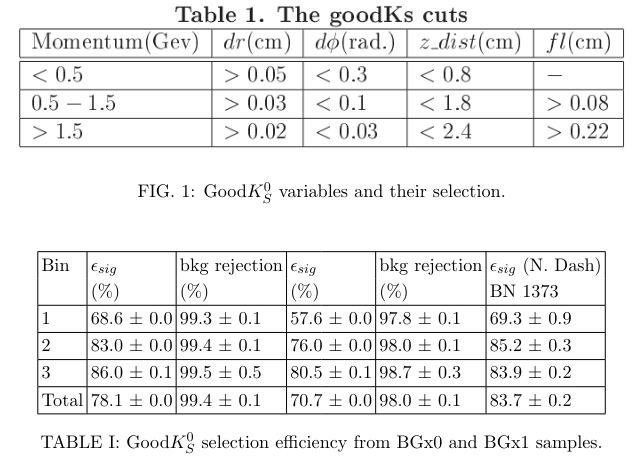
\includegraphics[width=0.73\linewidth]{img/goodKshortcut.png}
    \end{figure}
\end{frame}

\begin{frame}{Тагирование $\Lambda_c$}
    \begin{equation}
        F(x, args) = f_{\text{continuum}} + f_{\text{signal}} + f_{\text{back ground}}
    \end{equation}
    
    \begin{equation}
        f_{\text{continuum}}(x) = \exp\inner{\cfrac{x-\mu}{\lambda}} + a_0 + a_1 \cdot x
    \end{equation}
           
    \begin{equation}
        f_{\text{signal}}(x) = G(x; M_{\Lambda_c}, \sigma_1) + G(x; \mu_2, \sigma_2) + G(x; \mu_3, \sigma_3)
    \end{equation}

    \begin{equation}
        f_{\text{back ground}} = f_{\text{signal}}(x) \circledast \inner{\sqrt{x-M_\pi}\cdot\theta\inner{x-M_\pi}\cdot c_1 + \sqrt{x}\cdot\theta\inner{x}\cdot c_2}
    \end{equation}
\end{frame}


\begin{frame}{Тагирование $\Lambda_c$ на MC}
    \begin{figure}[H]
        \centering
        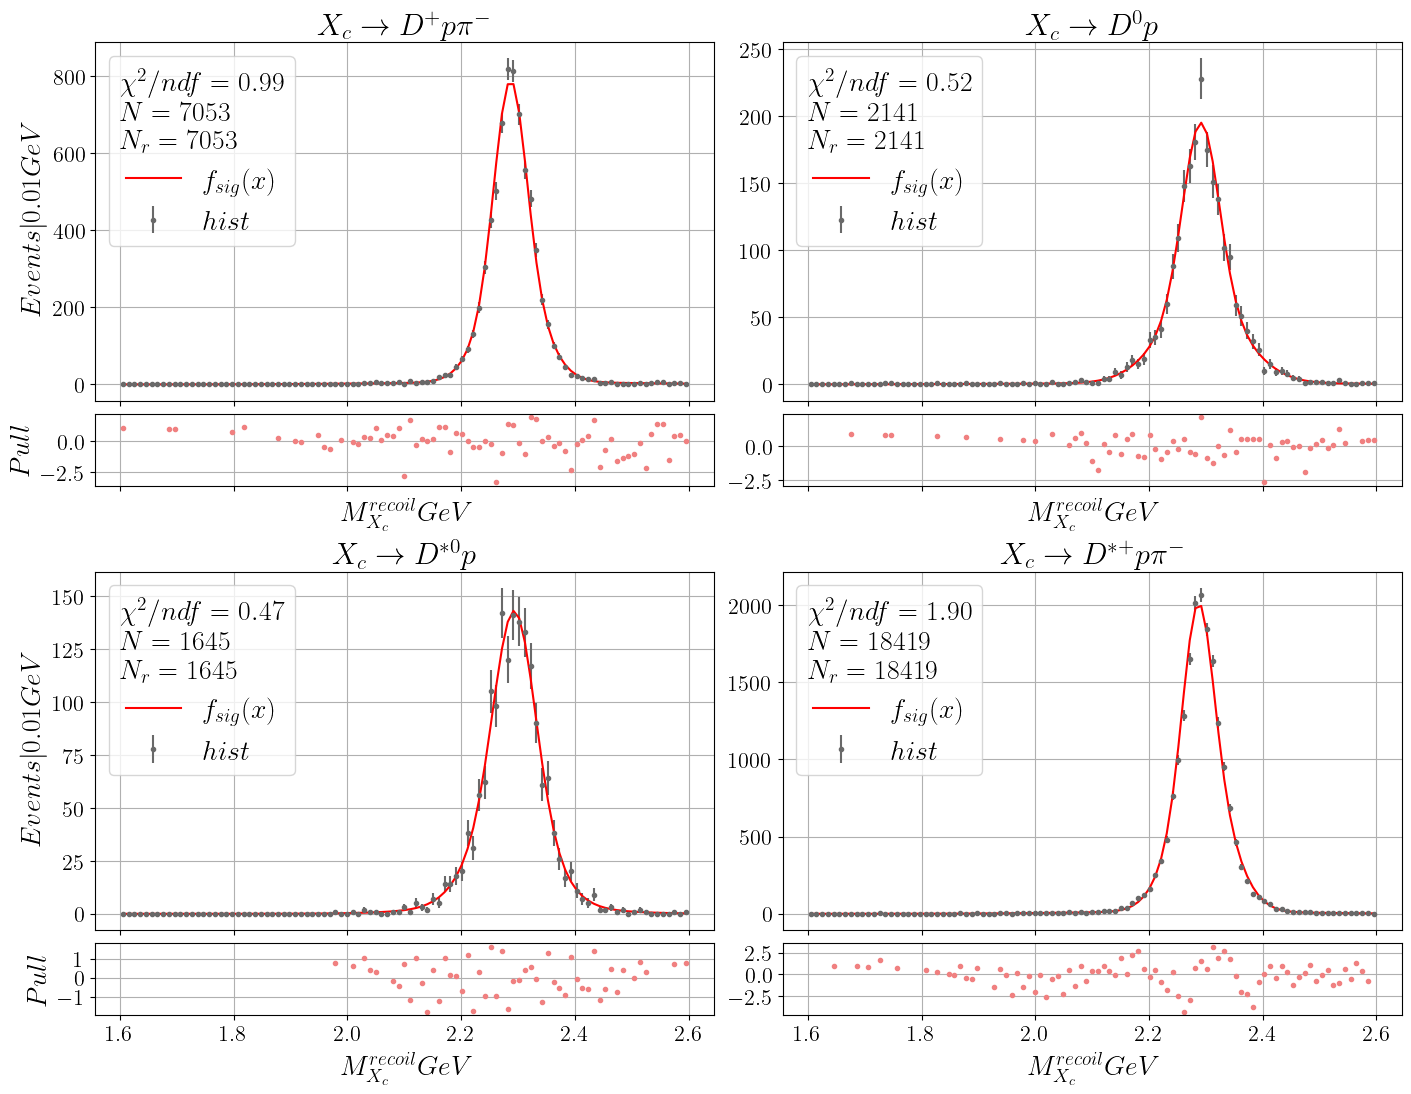
\includegraphics[width=0.74\linewidth]{img/MC_sig_fit.png}
    \end{figure}
    \begin{equation*}
        f_{\text{signal}}(x) = G(x; M_{\Lambda_c}, \sigma_1) + G(x; \mu_2, \sigma_2) + G(x; \mu_3, \sigma_3)
    \end{equation*}
\end{frame}

\begin{frame}{Тагирование $\Lambda_c$ на MC}
    \begin{figure}[H]
        \centering
        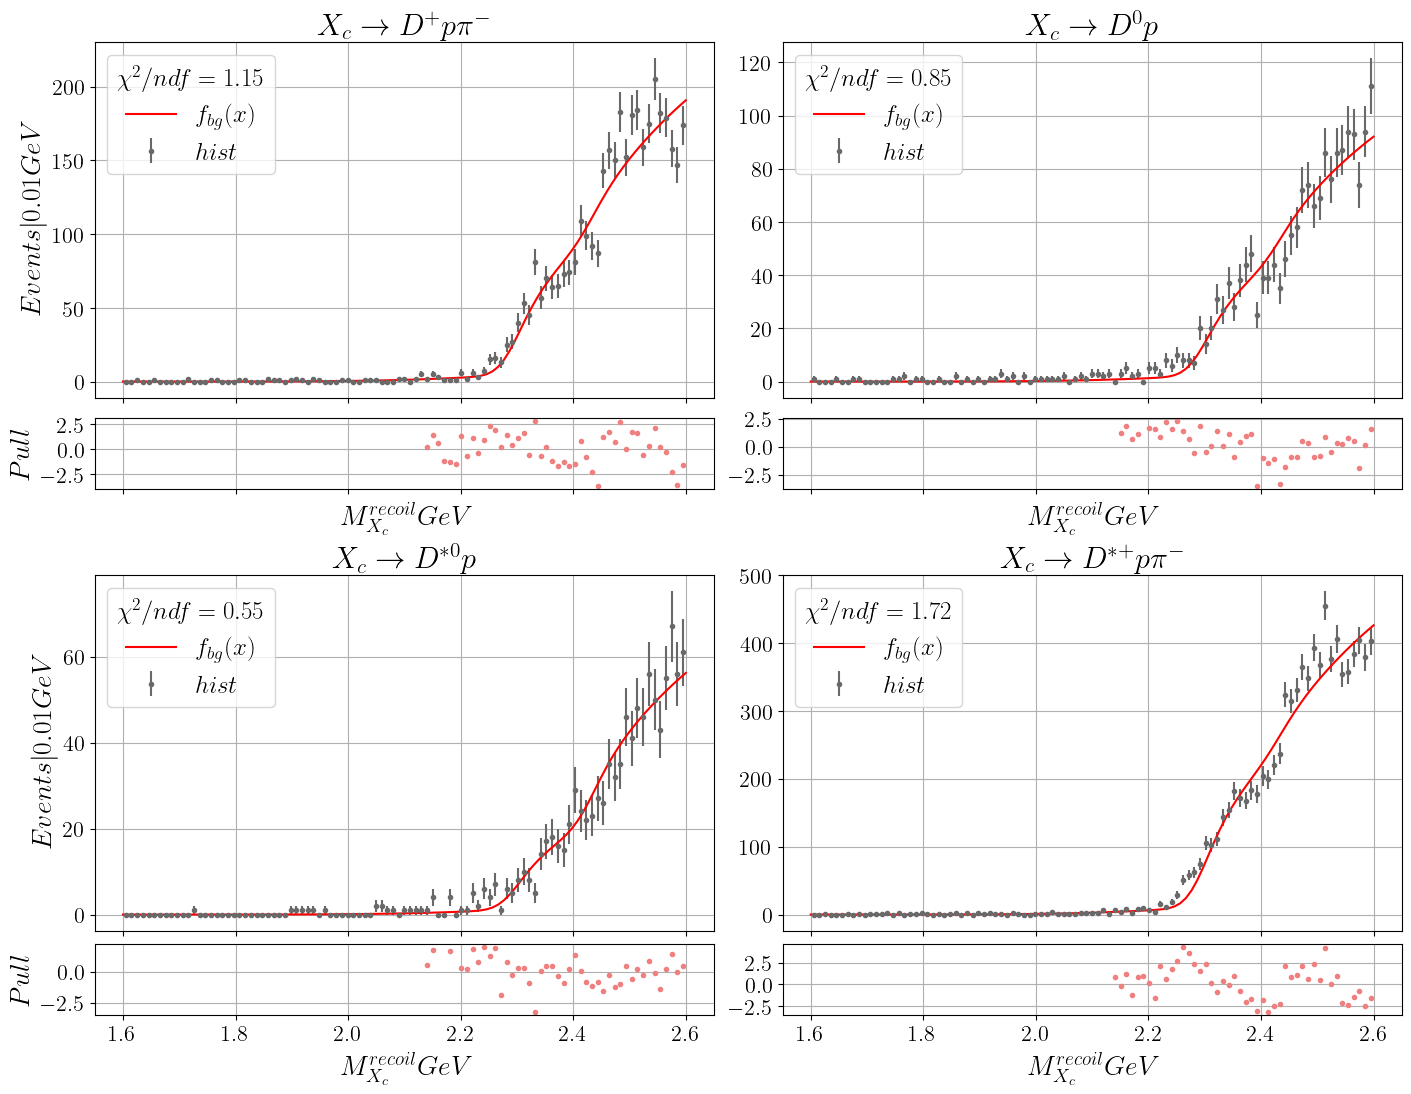
\includegraphics[width=0.74\linewidth]{img/MC_sqr_bg_fit.png}
    \end{figure}
    \begin{equation*}
        f_{\text{back ground}} = f_{\text{signal}}(x) \circledast \inner{\sqrt{x-M_\pi}\cdot\theta\inner{x-M_\pi}\cdot c_1 + \sqrt{x}\cdot\theta\inner{x}\cdot c_2}
    \end{equation*}
\end{frame}

\begin{frame}{Тагирование $\Lambda_c$ на MC}
    \begin{figure}[H]
        \centering
        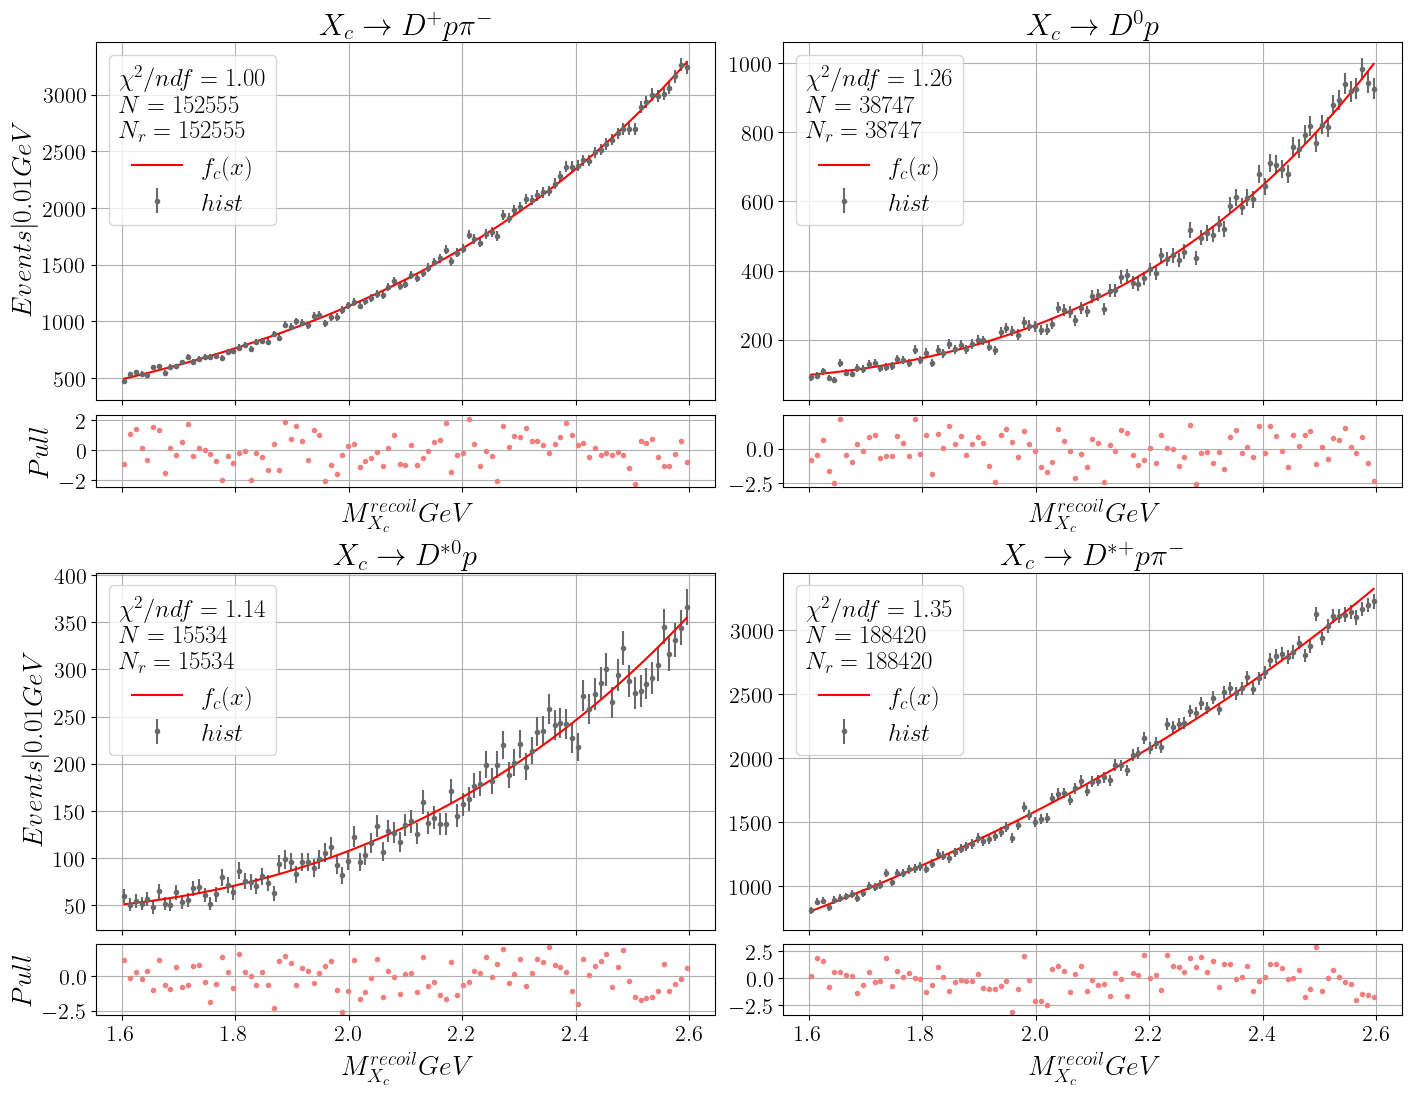
\includegraphics[width=0.73\linewidth]{img/MC_comb_fit.png}
    \end{figure}
    \begin{equation*}
        f_{\text{continuum}}(x) = \exp\inner{\cfrac{x-\mu}{\lambda}} + a_0 + a_1 \cdot x
    \end{equation*}
\end{frame}

\begin{frame}{Тагирование $\Lambda_c$ на Data}
    \begin{figure}[H]
        \centering
        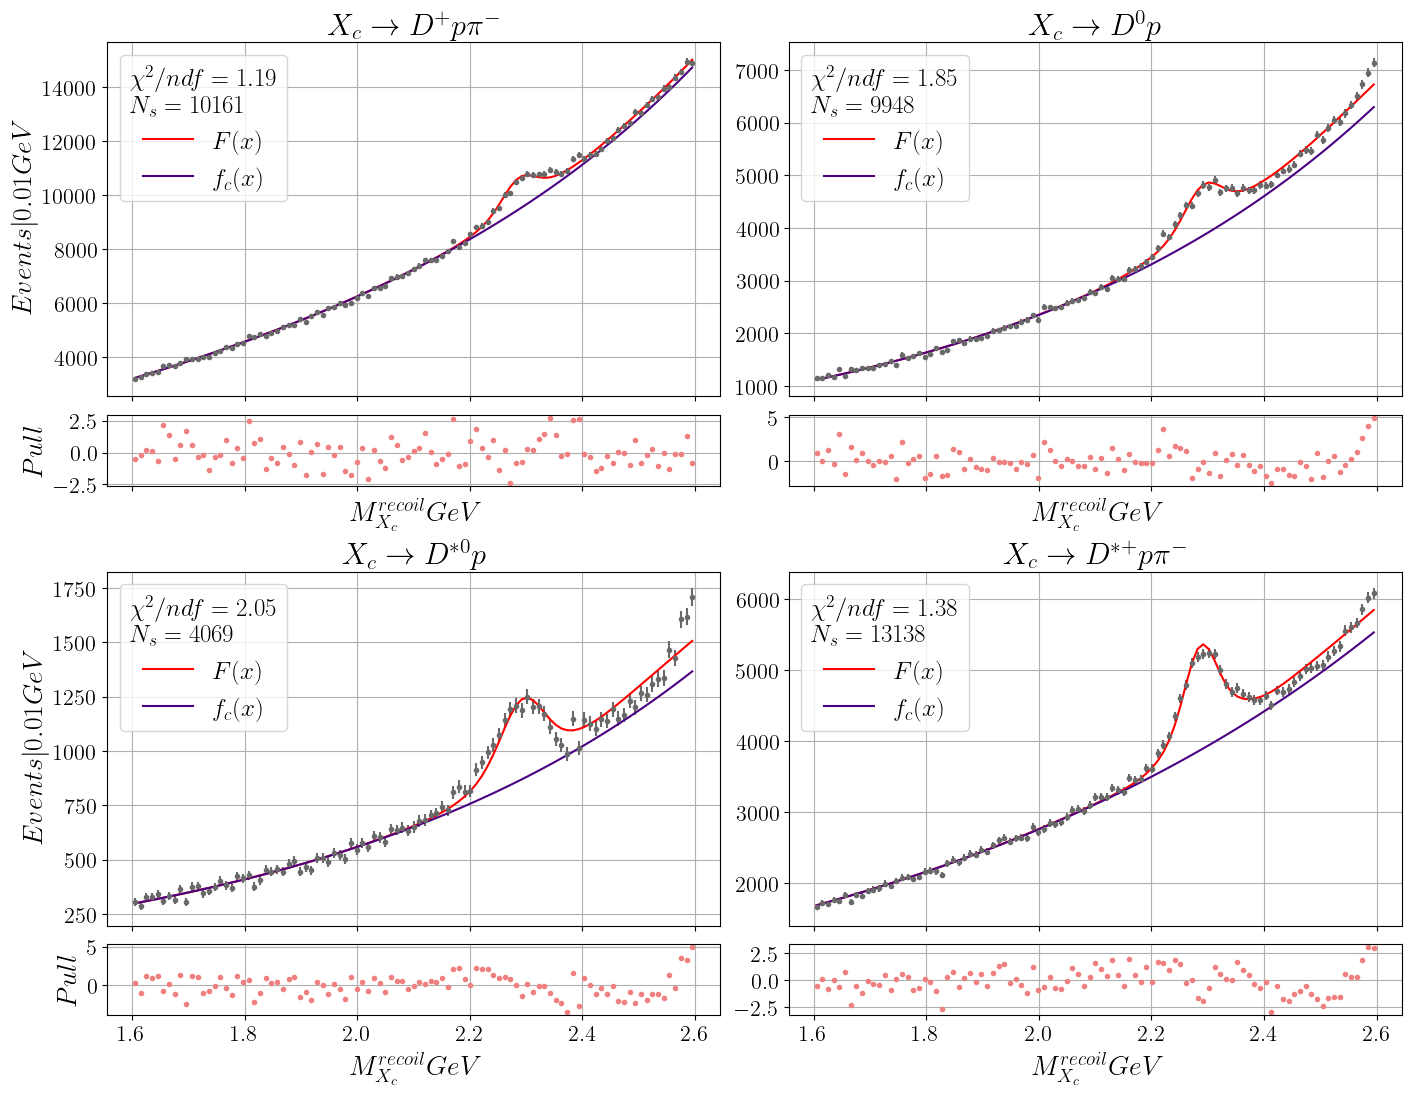
\includegraphics[width=0.73\linewidth]{img/fit_data.png}
    \end{figure}
    \begin{equation*}
        F(x, args) = f_{\text{continuum}} + f_{\text{signal}} + f_{\text{back ground}}
    \end{equation*}
\end{frame}

\begin{frame}{Сравнение с С. Приваловым}
    \begin{figure}[H]
        \centering
        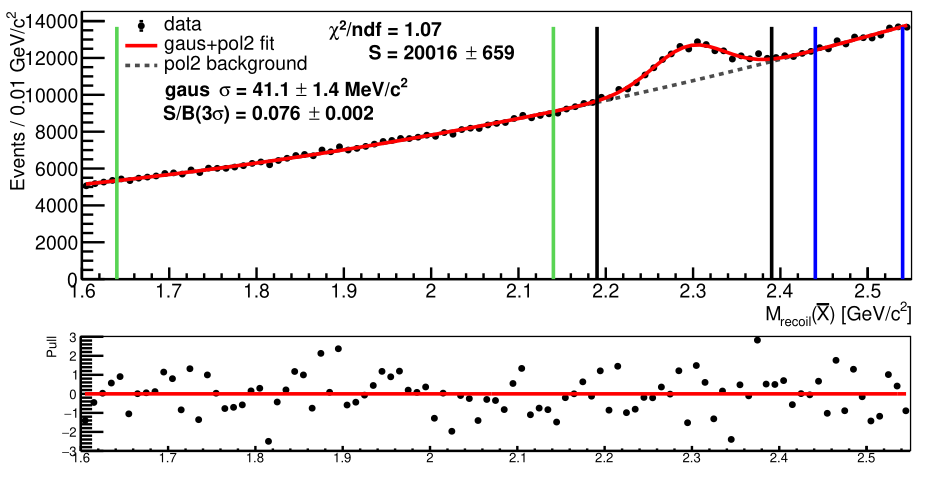
\includegraphics[width=0.73\linewidth]{img/priv_res.png}
    \end{figure}
\end{frame}



%\begin{frame}{Полная реконструкция}
%    \begin{columns}
%        \begin{column}{0.33\textwidth}
%            В изучаемой выборке:
%            \begin{equation*}
%                \Lambda_c^- \to \Lambda e^- \nu_e ; \ \Lambda \mu^- \nu_\mu 
%            \end{equation*}
%        \end{column}
%        \begin{column}{0.33\textwidth}
%            В пробной выборке :
%            \begin{equation*}
%                \Lambda_c^- \to \bar p K^+ \pi^-
%            \end{equation*}            
%        \end{column}
%        \begin{column}{0.33\textwidth}
%            В референсной:
%            \begin{equation*}
%                \Lambda_c^- \to \Lambda \pi 
%            \end{equation*}
%        \end{column}
%    \end{columns}
%    \begin{columns}
%        \begin{column}{0.5\textwidth}
%            \begin{itemize}
%                \item $z_{dist}\inner{\Lambda} > 1 cm$
%                \item $L(e, \mu) > \infig{0.01, 0.1}$
%                \item $\abs{P_e} > 0.6 GeV$
%                \item $\abs{P_\mu} > 1 GeV$
%            \end{itemize}
%        \end{column}
%        
%        \begin{column}{0.5\textwidth}
%            \begin{itemize}
%                \item $D^*\to D ... : \abs{M_{D*} - M_D} > 155 MeV$
%                \item $r_{dist}\inner{e, \mu} > 2 cm$
%                \item $N_{charged} <= 1$
%            \end{itemize}
%        \end{column}
%    \end{columns}
%\end{frame}



\end{document}